\documentclass{book}
\usepackage{graphicx} % Required for inserting images
\usepackage[utf8]{inputenc}
\usepackage{glossaries}
\usepackage{hyperref}


\title{Huw's Big Book of Linux}
\author{Huw Coverdale Jones}
\date{April 2023}

\begin{document}

\maketitle

\tableofcontents
\printglossaries

\chapter{Introduction - What is
Linux and Why Use it?}

\section{What is it?}
Once upon a time, there was a period where Windows may have faced some competition as the main Operating system for computers. Apple was broadly affordable, at least at primary schools in North Lincolnshire, and UNIX was operating on several systems. The NeXT Cube was running an OS made by Stephen Jobsworth (colloquially known by his stage name, Steve Jobs), and that was used by Tim Berners-Lee to invent the world wide web protocol, leading to the social phenomenon known by many as the internet. This means Twitter is his fault by the way.

Among this brave new multiple OS world, there lived in Fenno-Swede geek named Linus Torvalds. In his immortal words he said "I'm doing a (free) operating system (just a hobby, won't be big and professional like gnu) for 386(486) AT clones." After this, he took the basics of UNIX, made his own little system, and years later caused self indulgent geeks to be even less welcome at parties. 

Since then Linux has spiraled into many directions, all of which are definitely positively correlated with having lots of friends and being sexually active. Linux Mint and Ubuntu serve as free versions of MacOS, while Kali Linux is for people who hack for a living, or have just seen Mr Robot. Tails OS, Porteus, and Slack serve as computers that you can carry in your pocket on a USB stick. This, of course relies on finding a computer you can put said USB into, but even geeky past-times require marketing jargon these days.

For more technical explanations of what it is, use google. It's literally a free computer system that anyone can download, there's tons of info. Now, why use it?

\section{Why use it?}

There are many reasons to use Linux, just ask your local Games Workshop employee. The main ones are simple; it is often more lightweight than its commercial rivals, can be adapted to fit many functions, and it's pretty much always free. 

So, the first point; "lightweight" means "doesn't have too much bloated stuff that slows  down your hardware," in this case. This is far from universally true to Linux. For example, Kali uses plenty of RAM, and Ubuntu is often the first to add new graphical features, which some YouTubers claim pushed them to Linux Mint to avoid slowdown. However, there are many Linux distributions that use effective, but not cutting edge, features sparingly. The result varies, but can include extending the speed of a newer computer, or restoring an older computer to useability. I once used a "micro-distro" to speed up a clean room computer at a pharmaceutical firm, which was using a new version of windows on a fairly old hardware set up. It worked, but that  he IT department disliked it. Anyway, result is that certain distributions can extend your laptop's lifespan. The Laptop I'm writing this on is 8 years old, and runs Bodhi Linux, and works just fine.

Second, Linux is very adaptable. Most Linux distributions have some form of customisation available at installation. Some are also designed with specific features and applications in mind. As mentioned, Kali Linux is made with Penetration Testing in mind. That is, it comes with a series of hacking tools, and a lot of personal security features. Ubuntu has Edubuntu, a version compiled with teachers in mind, coming with a bundle of teaching software. It also has several other specialist versions, such as Ubuntu Studio for creatives, and Ubuntu Kylin, which is optimised for Chinese speakers. The Extreme examples of this are Arch Linux and Gentoo; The first of these examples requires you to make every minor decision about its form when you install it. The Second is specifically sold on the same grounds, with the specific aim of optimising your computer for a specific application. 

Finally, as highlighted earlier; by and large Linux is Free. MacOS is also a UNIX offshoot, and so is BSD, which you've never heard of, and I refuse to comment further on. Linux gives its Kernel (computer word for ... well something) to a series of free operating systems, most of which are compatible with a huge range of hardware. Ubuntu makes its money byhadoing contract work for comp hanies that want to run one of its flavours on their systems. Raspberry Pi sells their hardware, but their OS is freely available. In short, this means you have options. Therefore, you can easily experiment and, as long as you make backups, you won't need to worry about losing anything.

Next up, dear reader, we're going to look at where to start.

\chapter{Getting Started}
So, as I mentioned earlier, there are literally hundreds of operating systems based on the Linux Kernel. This chapter is an unfriendly and irreverent guide to picking one of those, and getting it up an running. 


\section{Start With an Easy Mode Linux}

Linux is more accessible than ever, unlike in the 90s when the drummer from Blur told you to get it before anyone had broadband. Starting out in Linux, it's advisable to go for an easy mode distro. Think of it as being like when you start a programming language with a "Hello World". 

So, there are a few of these, with many being invented and coded with this specific goal in mind. Generally, you can't go too far wrong with the Big U, Ubuntu. I was going to call it the Super U, but that's a collection of supermarkets in France. Anyway, Ubuntu has a large install base, comes with your basic software and is pretty easy to use. Many other beginner Linuxes are based on it, like Linux Mint, and Pop OS. It's based on Debian, but that's a story for another day, I just really wanted to highlight how much stuff is based on other stuff when you're talking about Linux. If you dislike white people making use of the languages of Central and Southern Africa (Google Ubuntu and realise how clever that joke is), you can get Manjaro or Peppermint.

Once you've picked your poison, you need to install.

\section{Installation - The Basics}
So, let's install Linux, because we don't want to settle down and get married anyway. 

To do so, you will need:

\begin{itemize}
    \item A USB key
    \item A computer
    \item Some patience, especially if you decided to start with Arch.
\end{itemize}

This is it, but you can have a cup of tea or coffee too. Keep it away from the computer, though. Anyway, on to the process;


\begin{enumerate}
    \item Turn on your computer normally.
    \item Ensure it is on a reliable internet connection, this comes up later.
    \item Log in and open a browser, then go to your chosen Distro's website. 
    \item It almost certainly has a link that says "install" or "download" in friendly bold letters. If not, send them an email and tell them to get a marketing expert to look over their webpage.
    \item This will probably lead to a page with  few options, for example, on the Ubuntu homepage (at the time of writing) it looks like this:
    
    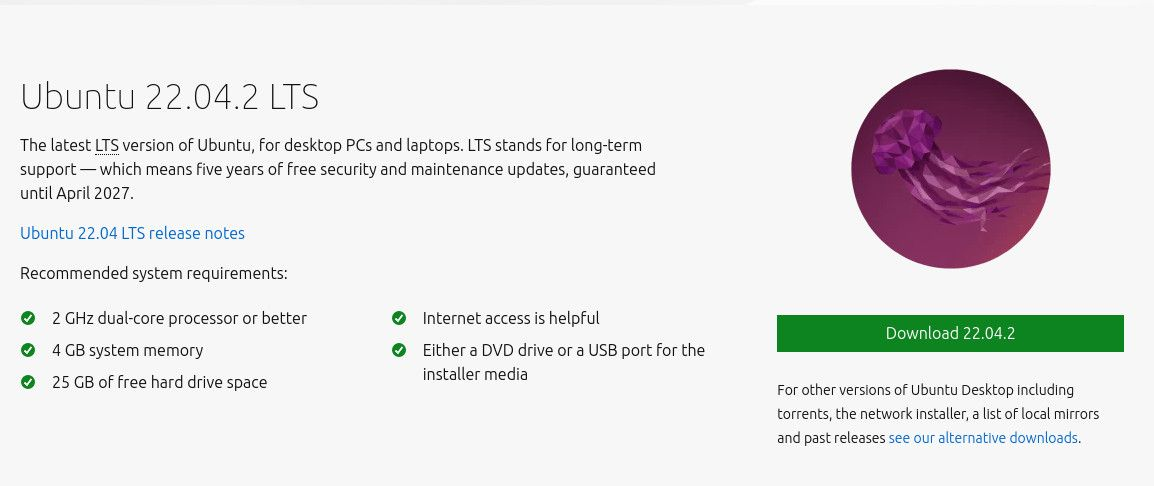
\includegraphics[scale=0.3]{2204.jpg}

    but then has this underneath:

    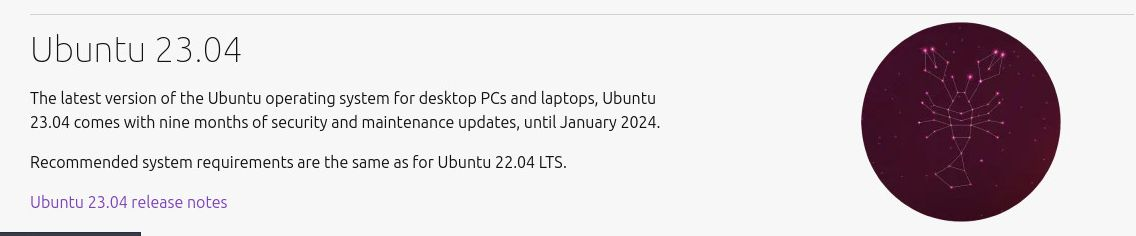
\includegraphics[scale=0.31]{2304.jpg}
    This is to enable you to choose between the Long Term Supported Release, and the latest one. The difference is which features it has, but also the older one may be just a bit more stable. Like how one of your parents is slightly more patient than the other.

    \item Click a link and a \verb|.iso| file will download. This is an image, basically a copy of the software you want. 
    \item Now, you need a way to make that into a bootable/installable USB image. There are a few, but a lot only work on Windows, so I recommend balenaEtcher (google it, I'm not your mum) which works on Mac, Windows, and Linux. 
    \item Download it and open it. In balenaEtcher, it looks like this:

    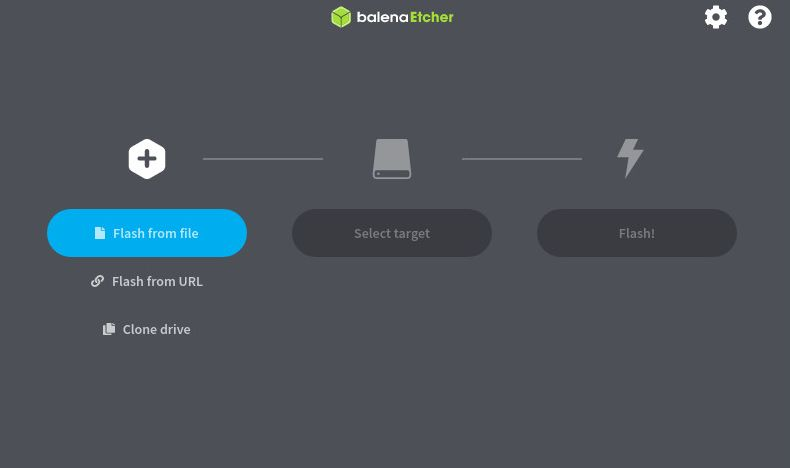
\includegraphics[scale=0.5]{balena.jpg}
    and to be honest this is pretty standard across the board for these softwares. 
    \item Insert your USB and make sure it appears on your computer. This will be important later.  

    \item   Select "Flash from file" or equivalent. A window will open.
    \item Locate the \verb|.iso| from step 5, and select it. 
    \item Click "Select target" or whatever it's called when you ignored my Balena advice. 
    \item Select the USB your inserted in step 8. 
    \item Click "Flash!".
    \item Ignore the obligatory "this will wipe the drive," message, unless you don't want it to. If you don't want it to, pick another USB stick, obviously.
    \item This will take some time, but not too much. When it tells you it is successful, close it. 
    \item Now we get to the hard part, which is booting into the USB. Restart your computer.
    \item As soon as your computer turns off, hold down the boot options key. This can be so many things, but Esc, F2, F10, or F12 are apparently common, according to a Linux blog I read once. 
    \begin{itemize}
        \item NOTE: Since windows 10, there has been an advanced restart option that enables this to be done automatically. I've used Linux since 2011, though, so you need to Google that again, \#sorrynotsorry. 
    \end{itemize}

    \item If all goes well, something like this should appear;
    
    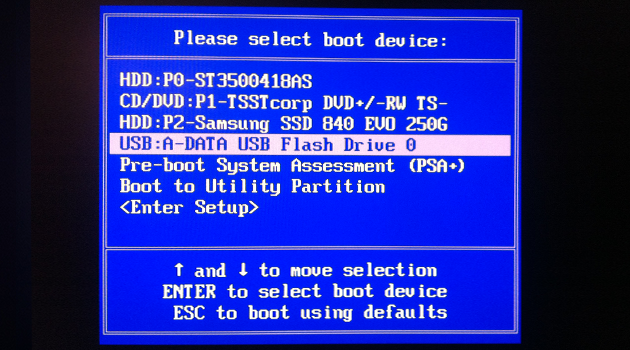
\includegraphics[scale=0.4]{options.png}

    If all did go well, skip to step 
    
    \item Unfortunately, it is possible all will not go well. Some manufacturers have gotten good at defending their proprietary systems. In this case, reboot and hold the advertised "setup" key. With PCs, You should be able to find something that resembles this:

    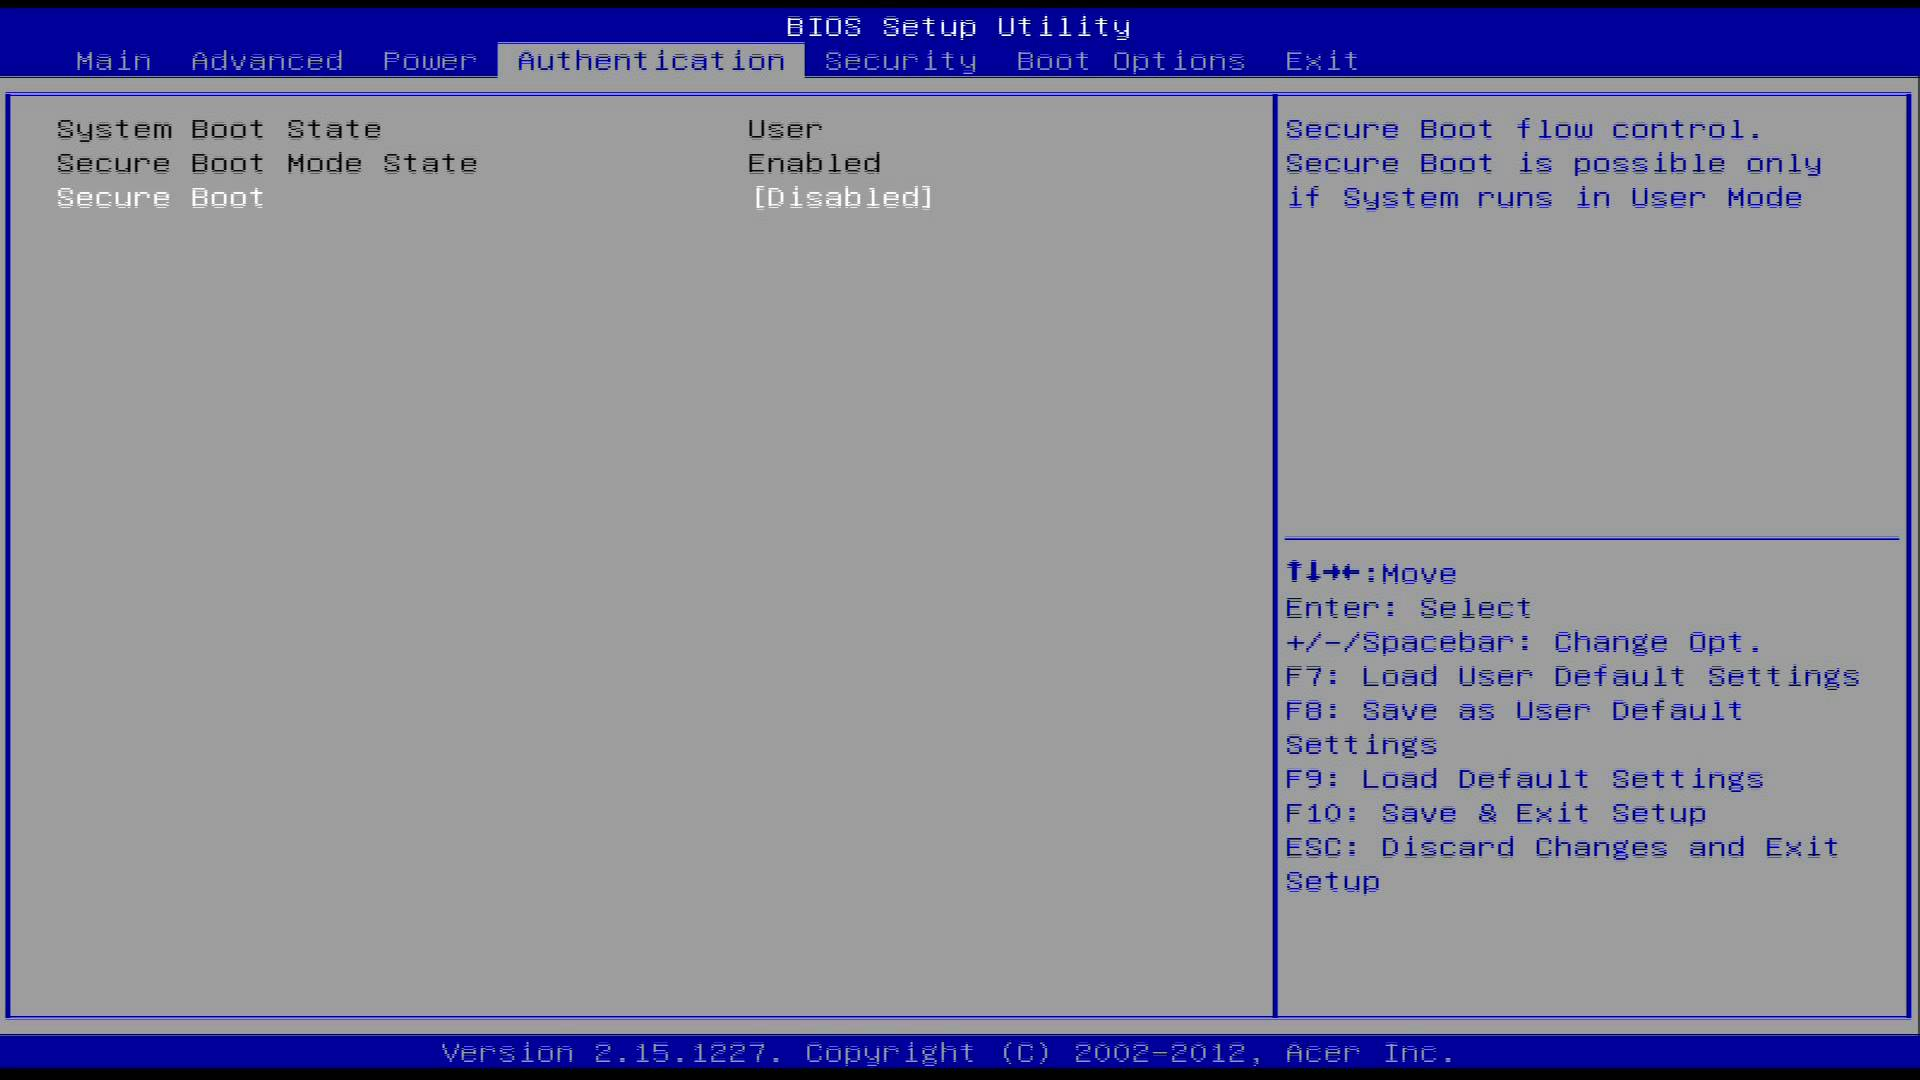
\includegraphics[scale=0.17]{secboot.jpg}
    
    Disable Secure boot, and reboot again, making sure to hold the required button and boot into the USB.
    I've never done this from Mac, because I'm too cool for well designed and well marketed software. However, \href{https://www.makeuseof.com/tag/install-linux-macbook-pro/} {MakeUseOf} says you can fix this with \href{https://sourceforge.net/projects/refind/}{rEFInd,} a software for undoing boot security on Mac. I included links this time, so calm down. 
    \item You should now be "in Linux" when the computer finishes start up. 
    \item No matter your chosen distro, unless it's a USB only one, you will get something like this:
    
    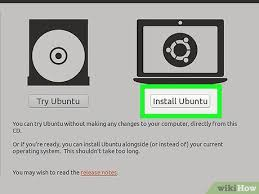
\includegraphics{ubs.jpeg}

    Click the "Install," unless you're having second thoughts. 

    \item The system will probably ask if you want to erase the whole system and replace it with Linux. In this tutorial, you do, I'll cover Dual Booting later.
    \item A wizard will open, inviting you to pick keyboard layout, geographical location and several other things. It's also quite likely to ask about installing from online. If you have the secure and reliable internet connection from Step 2, say "Sure, why not?" etc.
    \item Select what yourt heart desires and let the process finish. 
    \item Congrats! You're now an annoying alternative lifestyle human being.
\end{enumerate}

Foolishly, I mentioned Dual Booting earlier. I'll try and summarise that next.

\section{So You've Decided to Keep Windows - Dual Booting}

Jumping to a Linux only lifestyle can be a very intimidating prospect; what will you tell your parents? How will you explain the lifestyle to your kids? Well, fear not, there is an option to make your computer have two operating systems, operating separately. That way you can still use the large variety of established windows products AND their open source equivalents!  The possibilities are not endless, but there are at least two. 

So, here's what you need:

\begin{itemize}
    \item A USB key
    \item A computer
    \item balenaEtcher again
    \item More patience than last time.
\end{itemize}

Once again, I've never done this on Mac, so this guide starts with the assumption of a Windows machine. This process should work for windows 10 and 11. Also, for simplicity's sake, this is based on an Ubuntu installation again. While it varies, this is actually quite similar across distro types in my experience, but everyone starts with something Ubuntu like. 

Let's begin; 

\begin{enumerate} 
    \item If you haven't already, disable secure boot. 
    \item Turn on and log into your computer as normal. 
    \item Download the Ubuntu of your choice, and flash to your USB.
    \item The potentially dangerous bit starts here; Open the windows menu and search for \verb|Disk Management|, then open it. 
    \item In both Windows 11 and 10 (also 7 and 8!) it looks like this:

    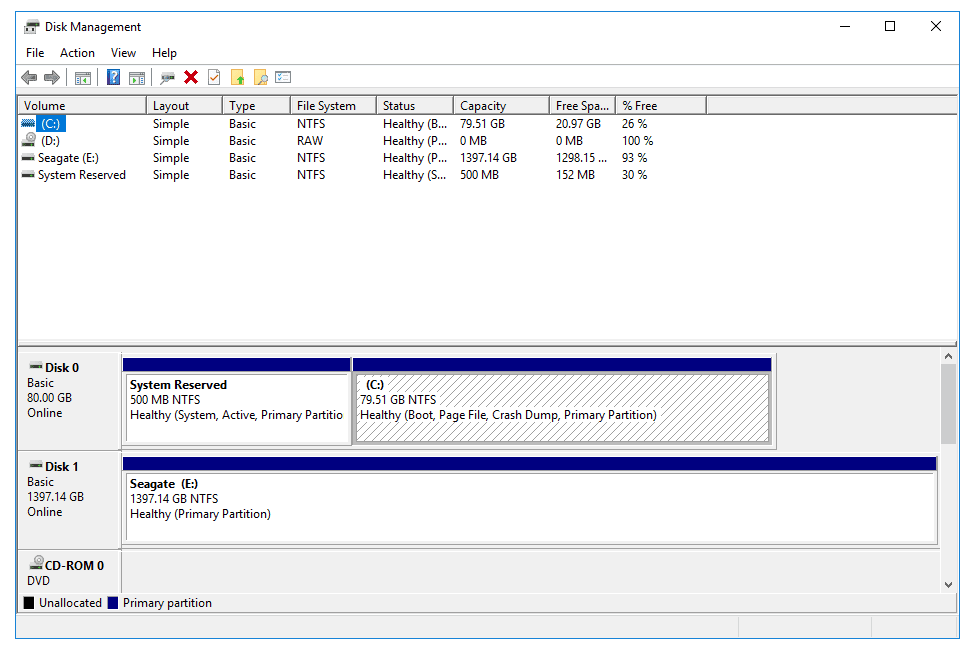
\includegraphics[scale = 0.3]{dmgmt.png}

    \item You need to shrink one of these bad boys. Your target is \verb|C:|. Right click it, then select \verb|Shrink Volume|.
    \item Shrink it down to the amount you now want to be set aside for your Linux play space. It may ask for the number in MB, not GB. 1024 MB is GB on computers, because reasons. Most blogs I've read suggest around 12GB minimum. However, as long as you shrink by 12GB or more, it's really up to you. 
    \item Reboot into the USB. As this is windows 10/11, you can do it by holding shift, then selecting \verb|Restart|. 
    \item A reboot options blue screen (of life, fortunately) will appear, with the option \verb|Use a device| then your USB drive. 
    \item You'll reboot into a handsome menu like this: 

    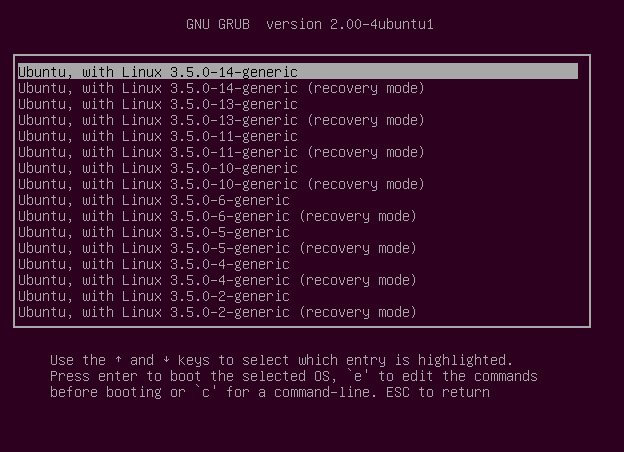
\includegraphics[scale = 0.5]{wubs.png}

    Just press enter    
    \item Now the choice to try or install Ubuntu will re appear. Select install again. 
    \item A window will appear with the option to \verb|Install Ubuntu alongside Windows Boot Manager|, select this.
    \item You should get this window:

    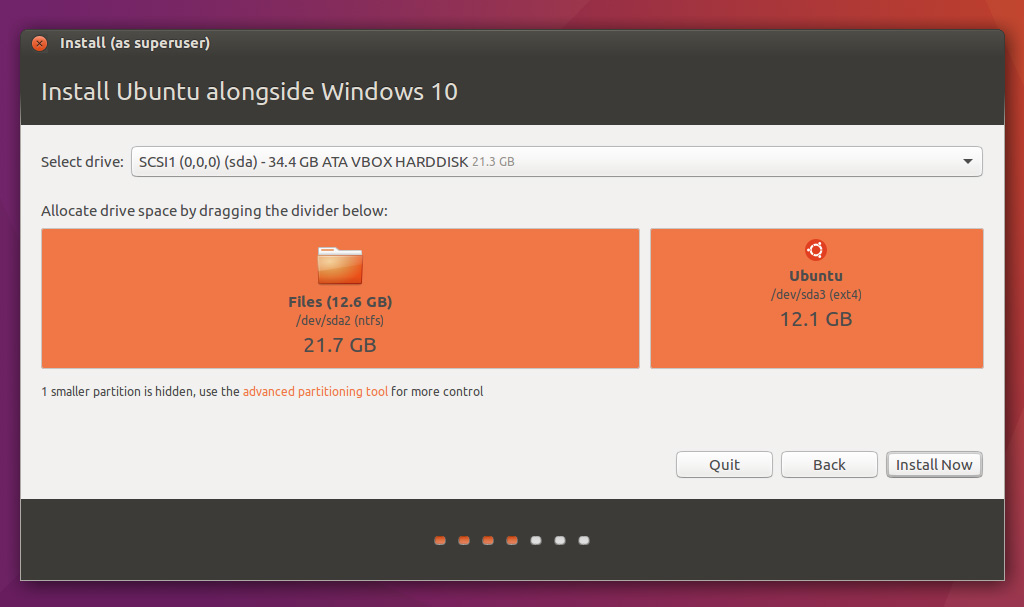
\includegraphics[scale = 0.4]{partit.jpg}
    
    This enables you to change the allocation of space for Linux. As standard, it has probably picked the GB you put aside earlier, but can be adjusted.
    \item Select \verb|Install Now| to make that part of your drive into the Linux space. It will automatically make a space for Linux, and put aside 2GB for swap space. 
    \item Follow the installation wizard step by step.
    \item Once finished, you have Ubuntu set up, but Windows still in tact.
    \item Now, when you restart, the handsome menu will reappear. As standard, it will have a countdown, after which Ubuntu will start. Pressing the arrow keys will stop this, enabling you to select Windows, if desired. 


\end{enumerate}

There you go, now you have both, and it's up to you to decide what to do with it. 


\chapter{What Next? - Specialist Applications}
\end{document}

